\section{p-n junctions and diodes}
\title{p-n junctions and diodes}  

\begin{frame}[plain]
    \titlepage
\end{frame}

%%%%%%%%%%%%%%%%%%%%%%%%%%%%%%%%%%%%%%%%%%%%%%%%%%%%%%%%%%%%%
%% Introduction to the p-n junctions %%
%%%%%%%%%%%%%%%%%%%%%%%%%%%%%%%%%%%%%%%%%%%%%%%%%%%%%%%%%%%%%
\begin{frame}
    \frametitle{What have you learnt and what you will learn?}

	\begin{itemize}
		\item WHat you have learnt so far? 
		\begin{itemize}
			\item How do a material behave as a conductor, semiconductor and insulator?
			\item How the current flows in a semiconductor?
			\item Mathematics of the current flow in a semiconductor?
			\item Proerpties of a intrinsic and extrinsic semiconductors?
			\item What is doping and \textbf{individual properties of n-type and p-type semiconductors?}
	\end{itemize}
		\item What you will learn in this lecture?
	\begin{itemize}
		\item What is a p-n junction? \textbf{How n-type and p-type semiconductors work together?}
		\item What is the depletion region?
		\item What is the built-in potential?
		\item What is the forward and reverse bias?
		\item What is the current-voltage characteristics of a diode?
		\item What are the different types of diodes?
		\item What are the applications of diodes?
	\end{itemize}
\end{itemize}
\end{frame}

%%%%%%%%%%%%%%%%%%%%%%%%%%%%%%%%%%%%%%%%%%%%%%%%%%%%%%%%%%%%%
%% Band diagrams of p-n junction %%
%%%%%%%%%%%%%%%%%%%%%%%%%%%%%%%%%%%%%%%%%%%%%%%%%%%%%%%%%%%%%
\begin{frame}
    \frametitle{Band diagrams of p-n junctions}
	\begin{itemize}
		\item A p-n junction is formed when a p-type semiconductor and an n-type semiconductor are brought into contact.
		\item The energy band diagrams of a p-n junction can be represented as follows:
		\begin{itemize}
			\item Before contact: The energy bands of the p-type and n-type semiconductors are separate.
			\item After contact: The energy bands of the p-n junction align, creating a depletion or space charge region at the interface.
			\item The conduction band and valence band of the n-type semiconductor are higher in energy than those of the p-type semiconductor.
			\item The Fermi level of the n-type semiconductor is higher than that of the p-type semiconductor before contact.
			\item After contact, the Fermi level becomes constant across the junction, indicating thermal equilibrium.
		\end{itemize}
		\item The energy band diagram of a p-n junction can be represented as follows:
\end{itemize}
\end{frame}


%%%%%%%%%%%%%%%%%%%%%%%%%%%%%%%%%%%%%%%%%%%%%%%%%%%%%%%%%%%%%
%% Band diagrams of p-n junction %%
%%%%%%%%%%%%%%%%%%%%%%%%%%%%%%%%%%%%%%%%%%%%%%%%%%%%%%%%%%%%%
\begin{frame}
    \frametitle{Band diagrams of p-n junctions}
	\begin{figure}
		\centering
		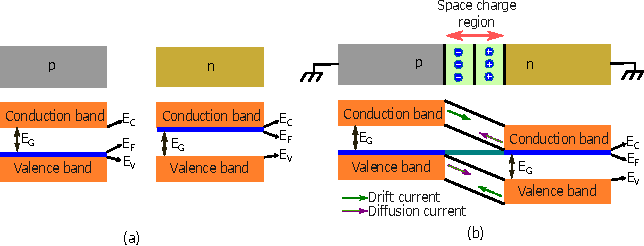
\includegraphics[width=0.8\textwidth]{fig/lec03/Band_diagram_all.pdf}
		\caption{Energy band diagram of a (a) discrete p and n (b) p-n junction.}
		\label{fig:pn_junction_all}
	\end{figure}
	\vspace{-0.5cm}
	\begin{itemize}
		\item The energy band diagram of a p-n junction shows the conduction band, valence band, and Fermi level of both the p-type and n-type semiconductors before and after contact.
		\item The depletion region is formed at the interface, where the majority carriers (holes in p-type and electrons in n-type) recombine, creating a region with no free charge carriers.
	\end{itemize}
\end{frame}


%%%%%%%%%%%%%%%%%%%%%%%%%%%%%%%%%%%%%%%%%%%%%%%%%%%%%%%%%%%%%
%% Band diagrams of p-n junction %%
%%%%%%%%%%%%%%%%%%%%%%%%%%%%%%%%%%%%%%%%%%%%%%%%%%%%%%%%%%%%%
\begin{frame}
	\frametitle{Band diagrams of p-n junctions}
	\begin{columns}
		\begin{column}{0.35\textwidth}
			\begin{itemize}
				\item \textbf{Step 1: Diffusion Due to Concentration Gradient}
				\begin{itemize}
					\item p-side: High hole concentration
					\item n-side: High electron concentration
					\item Result: Holes diffuse from p to n, electrons from n to p
				\end{itemize}
				\item \textbf{Step 2: Ions Left Behind → Space Charge}
				\begin{itemize}
					\item As mobile carriers leave, fixed ionized dopants remain:
					\begin{itemize}
						\item Negative acceptor ions in the p-region
						\item Positive donor ions in the n-region
					\end{itemize}
				\end{itemize}
			\end{itemize}
		\end{column}
		\begin{column}{0.7\textwidth}
			\begin{figure}
				\centering
				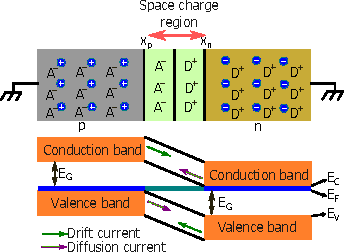
\includegraphics[scale=1.5]{fig/lec03/band_diagram_pn_junction_big.pdf}
				\caption{Energy band diagram of a p-n junction.}
				\label{fig:pn_junction}
			\end{figure}
		\end{column}
	\end{columns}
\end{frame}

%%%%%%%%%%%%%%%%%%%%%%%%%%%%%%%%%%%%%%%%%%%%%%%%%%%%%%%%%%%%%
%% Band diagrams of p-n junction %%
%%%%%%%%%%%%%%%%%%%%%%%%%%%%%%%%%%%%%%%%%%%%%%%%%%%%%%%%%%%%%
\begin{frame}
	\frametitle{Band diagrams of p-n junctions}
	\begin{columns}
		\begin{column}{0.5\textwidth}
			\begin{itemize}
				\item \textbf{Step 1: Diffusion Due to Concentration Gradient}
				\item \textbf{Step 2: Ions Left Behind → Space Charge}
				\begin{itemize}
					\item Creates a region with net charge — the \textbf{space charge region}
				\end{itemize}
				\item \textbf{Step 3: Built-in Electric Field Forms}
				\begin{itemize}
					\item The space charge generates an electric field $\mathcal{E}_{bi}$ (from n to p)
					\item This field opposes further carrier diffusion
				\end{itemize}
				\item \textbf{Step 4: Dynamic Balance Achieved}
				\begin{itemize}
					\item Eventually, drift current (due to $\mathcal{E}_{bi}$) balances diffusion current
					\item Net current = 0: system reaches \textbf{thermal equilibrium}
				\end{itemize}
			\end{itemize}
		\end{column}
		\begin{column}{0.5\textwidth}
			\begin{figure}
				\centering
				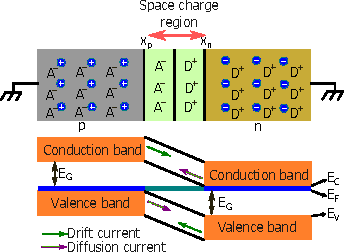
\includegraphics[scale=1]{fig/lec03/band_diagram_pn_junction_big.pdf}
				\caption{Energy band diagram of a p-n junction.}
				\label{fig:pn_junction}
			\end{figure}
		\end{column}
	\end{columns}
\end{frame}

%%%%%%%%%%%%%%%%%%%%%%%%%%%%%%%%%%%%%%%%%%%%%%%%%%%%%%%%%%%%%
%% Key insights in charge movement in p-n junctions %%
%%%%%%%%%%%%%%%%%%%%%%%%%%%%%%%%%%%%%%%%%%%%%%%%%%%%%%%%%%%%%
\begin{frame}
	\frametitle{Key Insights into Charge Movement}
	\begin{columns}
		\begin{column}{0.5\textwidth}
			\begin{itemize}
				\item Initial carrier flow is driven by \textbf{concentration gradients}, not electric forces.
				\item Opposite charges do not attract each other across the junction initially.
				\item The \textbf{electric field is a result of diffusion}, not the cause of it.
				\item The depletion region is characterized by:
				\begin{itemize}
					\item No free carriers
					\item Net space charge from fixed dopants
				\end{itemize}
				\item The system reaches an equilibrium defined by the \textbf{built-in potential} $V_{bi}$.
			\end{itemize}
		\end{column}
		\begin{column}{0.5\textwidth}
			\begin{figure}
				\centering
				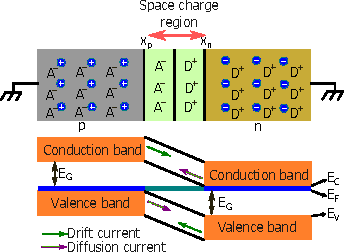
\includegraphics[scale=1]{fig/lec03/band_diagram_pn_junction_big.pdf}
				\caption{Energy band diagram of a p-n junction.}
				\label{fig:pn_junction}
			\end{figure}
		\end{column}
	\end{columns}
\end{frame}


%%%%%%%%%%%%%%%%%%%%%%%%%%%%%%%%%%%%%%%%%%%%%%%%%%%%%%%%%%%%%
%% Electric field intensity in space charge regions %%
%%%%%%%%%%%%%%%%%%%%%%%%%%%%%%%%%%%%%%%%%%%%%%%%%%%%%%%%%%%%%
\begin{frame}{Electric Field Intensity in the scpace charge region}
    \begin{itemize}
        \item The depletion region in a pn junction contains \textbf{uncompensated dopant ions} (donors in n-side, acceptors in p-side).
        \item This fixed charge distribution creates a \textbf{space-charge density} $\rho(x)$, giving rise to an electric field.
        \item According to \textbf{Poisson's equation}:
        \begin{equation}
            \frac{d^2 V}{dx^2} = -\frac{\rho(x)}{\varepsilon}
        \end{equation}
        where $V$ is the electrostatic potential and $\varepsilon$ is the permittivity.

        \item Integrating Poisson's equation yields the electric field:
        \begin{equation}
            \mathcal{E}(x) = \int_{x_p}^x \frac{\rho(x_n)}{\varepsilon} dx
        \end{equation}
        where $x_p$ is the reference point where $\mathcal{E}(x_p) = 0$.
    \end{itemize}
\end{frame}

%%%%%%%%%%%%%%%%%%%%%%%%%%%%%%%%%%%%%%%%%%%%%%%%%%%%%%%%%%%%%
%% Electric field intensity in space charge regions %%
%%%%%%%%%%%%%%%%%%%%%%%%%%%%%%%%%%%%%%%%%%%%%%%%%%%%%%%%%%%%%
\begin{frame}{Electric Field Intensity in the space charge region}
    \begin{itemize}
        \item \textbf{Electric field direction:}
        \begin{itemize}
            \item Points from n-side (positive charge) to p-side (negative charge).
            \item Corresponds to \textbf{negative field intensity} if potential decreases from n to p.
        \end{itemize}
        \item The electric field acts like an \textbf{internal dipole layer}, enabling the concept of \textbf{built-in potential} $V_0$.
		\item \textbf{Equilibrium condition:}
        \item At thermal equilibrium, i.e. the steady-state condition at a given temperature with no external excitations, the
		individual electron and hole currents flowing across the junctions are identically zero. Thus, for each type of
		carrier the drift current due to the electric field must exactly cancel the diffusion current due to the concentration
		gradient.
		\begin{equation}
			j_n = j_p = 0 \Rightarrow j_n + j_p = 0
		\end{equation}
		\item The total current density is given by:
		\begin{equation}
			j = j_n (\text{drift}) + j_p (\text{diffusion}) = q \left( \mu_n n \mathcal{E} + D_n \frac{dn}{dx} - \mu_p p \mathcal{E} - D_p \frac{dp}{dx} \right) = 0
		\end{equation}
    \end{itemize}
\end{frame}

%%%%%%%%%%%%%%%%%%%%%%%%%%%%%%%%%%%%%%%%%%%%%%%%%%%%%%%%%%%%%
% Built-in Voltage: Starting with Einstein Relation and Drift-Diffusion#
%%%%%%%%%%%%%%%%%%%%%%%%%%%%%%%%%%%%%%%%%%%%%%%%%%%%%%%%%%%%%
\begin{frame}{Built-in Voltage: Einstein Relation and Carrier Distribution}
    \begin{itemize}
        \item From the Einstein relation, the drift-diffusion equations become:
        \begin{align}
            j_n &= q \mu_n \left( n \mathcal{E} + \frac{kT}{q} \frac{dn}{dx} \right)  \\
            j_p &= q \mu_p \left( p \mathcal{E} - \frac{kT}{q} \frac{dp}{dx} \right) 
        \end{align}
        \item At equilibrium ($j_p = 0$), using integration of the expression inside the bracket gives:
        \begin{equation}
            p(x) = p(x_p) e^{-\frac{qV(x)}{kT}}
        \end{equation}
        \item With $V(x) = - \int_{x_p}^{x} \mathcal{E}(x') dx'$
        \item Similarly for electrons:
        \begin{equation}
            n(x) = n(x_n) e^{\frac{qV(x)}{kT}} 
        \end{equation}
        \item These distributions are referred to as the \textbf{Boltzmann distribution} under equilibrium.
    \end{itemize}
\end{frame}

%%%%%%%%%%%%%%%%%%%%%%%%%%%%%%%%%%%%%%%%%%%%%%%%%%%%%%%%%%%%%
% Built-in Potential Derivation
%%%%%%%%%%%%%%%%%%%%%%%%%%%%%%%%%%%%%%%%%%%%%%%%%%%%%%%%%%%%%
\begin{frame}{Derivation of Built-in Potential $V_{bi}$}
    \begin{itemize}
        \item Carrier product at any point:
        \begin{equation}
            n \cdot p = n_i^2 
        \end{equation}
        \item Built-in potential is given by:
        \begin{equation}
            V_{bi} = V(x_n) = \frac{kT}{q} \ln\left( \frac{p(x_p)}{p(x_n)} \right) = \frac{kT}{q} \ln\left( \frac{p(x_p) \cdot n(x_n)}{n_i^2} \right) 
        \end{equation}
        \item Assuming complete ionization at boundaries:
        \begin{equation}
            V_{bi} \cong \frac{kT}{q} \ln\left( \frac{N_A(x_p) \cdot N_D(x_n)}{n_i^2} \right) 
        \end{equation}
        \item This shows that $V_{bi}$ depends only on the doping levels and intrinsic carrier concentration.
        \item Important for setting the electrostatic barrier preventing further diffusion across the junction.
    \end{itemize}
\end{frame}

%%%%%%%%%%%%%%%%%%%%%%%%%%%%%%%%%%%%%%%%%%%%%%%%%%%%%%%%%%%%%
% Summary and insights in built-in potential
%%%%%%%%%%%%%%%%%%%%%%%%%%%%%%%%%%%%%%%%%%%%%%%%%%%%%%%%%%%%%
\begin{frame}{Key Insights from Built-in Potential Derivation}
    \begin{itemize}
		\item \textbf{1. Drift-Diffusion Balance at Equilibrium}
		\begin{itemize}
			\item Currents consist of drift + diffusion components.
			\item At equilibrium: $j_n = j_p = 0 \Rightarrow$ drift current = $-$ diffusion current.
		\end{itemize}

        \item \textbf{2. Carrier Densities Follow Boltzmann Distributions}
        \begin{itemize}
            \item $p(x) = p(x_p) e^{-\frac{qV(x)}{kT}},\quad n(x) = n(x_n) e^{\frac{qV(x)}{kT}}$
            \item Potential $V(x)$ governs spatial variation in carrier concentration.
        \end{itemize}

        \item \textbf{3. Mass Action Law Holds:} $n(x) \cdot p(x) = n_i^2$ \textit{everywhere in depletion region}

        \item \textbf{4. Built-in Voltage Expression:}
        \begin{equation}
            V_{bi} = \frac{kT}{q} \ln\left(\frac{N_A(x_p) \cdot N_D(x_n)}{n_i^2}\right)
		\end{equation}
        \begin{itemize}
            \item Depends only on doping densities and intrinsic carrier concentration.
            \item Sets up internal electrostatic barrier to prevent further diffusion.
        \end{itemize}

        \item \textbf{5. Interpretation:}
        \begin{itemize}
            \item \textit{Defines equilibrium energy band bending and barrier height.}
            \item \textit{Logarithmic dependence allows efficient doping control of $V_{bi}$.}
        \end{itemize}
    \end{itemize}
\end{frame}


%%%%%%%%%%%%%%%%%%%%%%%%%%%%%%%%%%%%%%%%%%%%%%%%%%%%%%%%%%%%%
% Biasing of p-n junctions
%%%%%%%%%%%%%%%%%%%%%%%%%%%%%%%%%%%%%%%%%%%%%%%%%%%%%%%%%%%%%
\begin{frame}{Biasing of p-n junctions}
	\textbf{All discussions in the previous slides were based on the assumption of thermal equilibrium and no external fields.} \\
	The behavior of a p-n junction can be controlled by applying an external voltage across the junction. \\
	\textbf{Biasing} refers to the application of an external voltage across a p-n junction to control its operation. The two main types of biasing are:
	\begin{columns}
		\begin{column}{0.5\textwidth}
			\begin{itemize}
				\item \textbf{Forward Bias:} Positive voltage applied to the p-side and negative voltage to the n-side.
			\end{itemize}
			\begin{figure}
				\centering
				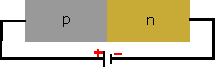
\includegraphics[scale=1]{fig/lec03/pn_forward_bias.pdf}
				\caption{Forward bias of a p-n junction.}
				\label{fig:forward_bias_pn_junction}
			\end{figure}
		\end{column}
		\begin{column}{0.5\textwidth}
			\begin{itemize}
				\item \textbf{Reverse Bias:} Positive voltage applied to the n-side and negative voltage to the p-side.
			\end{itemize}
			\begin{figure}
				\centering
				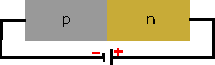
\includegraphics[scale=1]{fig/lec03/pn_reverse_bias.pdf}
				\caption{Reverse bias of a p-n junction.}
				\label{fig:reverse_bias_pn_junction}
			\end{figure}
		\end{column}
	\end{columns}
\end{frame}

%%%%%%%%%%%%%%%%%%%%%%%%%%%%%%%%%%%%%%%%%%%%%%%%%%%%%%%%%%%%%
% Reverse bias of p-n junctions
%%%%%%%%%%%%%%%%%%%%%%%%%%%%%%%%%%%%%%%%%%%%%%%%%%%%%%%%%%%%%

\begin{frame}{Reverse bias in a \textit{p-n} Junction}
    \textbf{Key Concept:} Reverse bias widens the depletion region and blocks majority carrier flow.
    \begin{itemize}
        \item \textbf{Biasing:} Negative terminal to $p$-side, positive to $n$-side (Fig. \ref{fig:reverse_bias_pn_junction}).
        \item \textbf{Effect:} Drives majority carriers (holes in $p$, electrons in $n$) \textit{away} from the junction.
        \item \textbf{Depletion Region:} Widens due to carrier drift, increasing the electric field barrier.
        \item \textbf{Steady State:} Cannot sustain continuous diffusion without replenishment $\Rightarrow$ nominally zero current.
        \item \textbf{Reverse Saturation Current $I_0$:}
        \begin{itemize}
            \item Small current due to minority carriers thermally generated.
            \item $I_0$ increases with temperature, but is \textit{independent} of applied reverse voltage.
        \end{itemize}
        \item \textbf{Physical Insight:} Potential barrier increases by $qV \Rightarrow$ blocks majority carriers, but allows minority carriers to flow.
		\item \textbf{Reverse Bias Breakdown:} If reverse voltage exceeds a critical value, breakdown occurs (Zener or avalanche breakdown).
    \end{itemize}
\end{frame}

%%%%%%%%%%%%%%%%%%%%%%%%%%%%%%%%%%%%%%%%%%%%%%%%%%%%%%%%%%%%%
% Forward bias of p-n junctions
%%%%%%%%%%%%%%%%%%%%%%%%%%%%%%%%%%%%%%%%%%%%%%%%%%%%%%%%%%%%%

\begin{frame}{Forward bias in a \textit{p-n} Junction}
	\begin{columns}
		\begin{column}{0.7\textwidth}
			\textbf{Key Concept:} Forward bias lowers the potential barrier and allows majority carrier injection.
			\begin{itemize}
				\item \textbf{Biasing:} Positive terminal to $p$-side, negative to $n$-side.
				\item \textbf{Effect:} Lowers the junction barrier height by $qV$, aiding carrier diffusion.
				\item \textbf{Depletion Region:} Narrows, reducing the internal electric field.
				\item \textbf{Carrier Movement:}
				\begin{itemize}
					\item Holes from $p$ move into $n$-side $\Rightarrow$ \textit{injected minority current}
					\item Electrons from $n$ move into $p$-side $\Rightarrow$ \textit{minority current in opposite direction}
				\end{itemize}
				\item \textbf{Current Flow:} Resultant current = sum of hole and electron minority currents.
				\item \textbf{Diode Equation:} $I = I_0 \left(e^{qV/kT} - 1\right)$ (derived later)
    	\end{itemize}
	\end{column}
		\begin{column}{0.3\textwidth}
			\begin{figure}
				\centering
				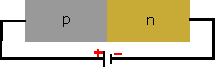
\includegraphics[scale=1]{fig/lec03/pn_forward_bias.pdf}
				\caption{Forward bias of a p-n junction.}
				\label{fig:forward_bias_pn_junction}
			\end{figure}
		\end{column}
	\end{columns}
\end{frame}

%%%%%%%%%%%%%%%%%%%%%%%%%%%%%%%%%%%%%%%%%%%%%%%%%%%%%%%%%%%%%
% Ohmic contacts in of p-n junctions
%%%%%%%%%%%%%%%%%%%%%%%%%%%%%%%%%%%%%%%%%%%%%%%%%%%%%%%%%%%%%

\begin{frame}{\textbf{Ohmic Contacts in \textit{p-n} Junctions}}
    \textbf{Definition:} \textit{Ohmic contacts} are special metal-semiconductor interfaces engineered to allow current to flow freely in both directions, without rectification behavior.

    \vspace{1em}
    \textbf{Key Assumptions:}
    \begin{itemize}
        \item In practical \textit{p-n} diodes, external bias is applied via metal contacts to both the $p$ and $n$ regions.
        \item These contacts create metal-semiconductor junctions — which, in general, could have their own contact potential.
        \item \textbf{Ohmic contacts} are designed to ensure:
        \begin{itemize}
            \item Contact potential remains \textbf{constant}, irrespective of current direction or magnitude.
            \item There is \textbf{no barrier to carrier flow} at the metal-semiconductor interface.
        \end{itemize}
    \end{itemize}
\end{frame}

\begin{frame}{\textbf{Ohmic Contacts in \textit{p-n} Junctions cont..}}
\textbf{Physical Insight:}
\textbf{Justification of Bias Assumption:}
\begin{itemize}
	\item Because the ohmic contacts are nonrectifying and the voltage drop across the bulk crystal is negligible,
	\item $\Rightarrow$ \textbf{Entire external bias appears across the \textit{p-n} junction barrier.}
	\item This simplifies analysis: bias voltage directly modifies the potential barrier height.
\end{itemize}
\textbf{Conclusion:}
\begin{itemize}
	\item Ohmic contacts are \textbf{essential} for accurate modeling of diode behavior under applied bias.
	\item They ensure that changes in applied voltage affect only the junction, not the metal-semiconductor interfaces.
\end{itemize}
\end{frame}


\begin{frame}{\textbf{Short-Circuited and Open-Circuited \textit{p-n} Junction}}
    \textbf{Physical Insight:} The behavior of a \textit{p-n} junction under short-circuit ($V = 0$) or open-circuit conditions ($I = 0$) reveals fundamental principles of equilibrium electrostatics and energy conservation.

    \vspace{0.7em}
    \textbf{Key Points:}
    \begin{itemize}
        \item When $V = 0$ is applied across the \textit{p-n} diode (Fig. \ref{fig:forward_bias_pn_junction} or Fig. \ref{fig:reverse_bias_pn_junction}), the junction is \textbf{short-circuited}.
        \item Under thermal equilibrium, this implies:
        \begin{itemize}
            \item Net current $I = 0$
            \item Junction potential $V_0$ remains unchanged.
        \end{itemize}

        \item \textbf{Energy conservation argument:}
        \begin{itemize}
            \item If current $I \neq 0$, metal wire heats up.
            \item No external energy source exists, so energy must come from \textit{p-n} bar $\Rightarrow$ thermal cooling of bar.
            \item \textbf{Contradiction:} Can't have metal heating and bar cooling simultaneously in equilibrium.
            \item \textbf{Conclusion:} $I = 0$
        \end{itemize}
	\end{itemize}
\end{frame}

\begin{frame}{\textbf{Short-Circuited and Open-Circuited \textit{p-n} Junction}}
	\begin{itemize}
	\item \textbf{Voltage Loop Consistency:}
	\begin{itemize}
		\item Total voltage drop across closed loop must be zero.
		\item $V_0$ is exactly compensated by contact potentials at ohmic contacts.
		\item Even if wire is cut, voltage drop remains zero.
	\end{itemize}

	\item \textbf{Implication:} $V_0$ cannot be measured directly by a voltmeter.
	\end{itemize}

	\vspace{0.7em}
	\textbf{Conclusion:} \textit{Built-in potential $V_0$ exists, but is internally balanced by metal-semiconductor junctions; it is not externally measurable.}
\end{frame}


\begin{frame}{The current components in a \textit{p-n} Junction}
\begin{columns}
		\begin{column}{0.225\textwidth}
	\textbf{Key Idea: Minority carrier injection under forward bias}
	\begin{itemize}
		\item When a forward voltage $V$ is applied:
		\begin{itemize}
			\item Holes are injected from $p$ to $n$ region.
			\item Electrons are injected from $n$ to $p$ region.
		\end{itemize}
	\end{itemize}
\end{column}
\begin{column}{0.775\textwidth}
	\begin{figure}
		\centering
		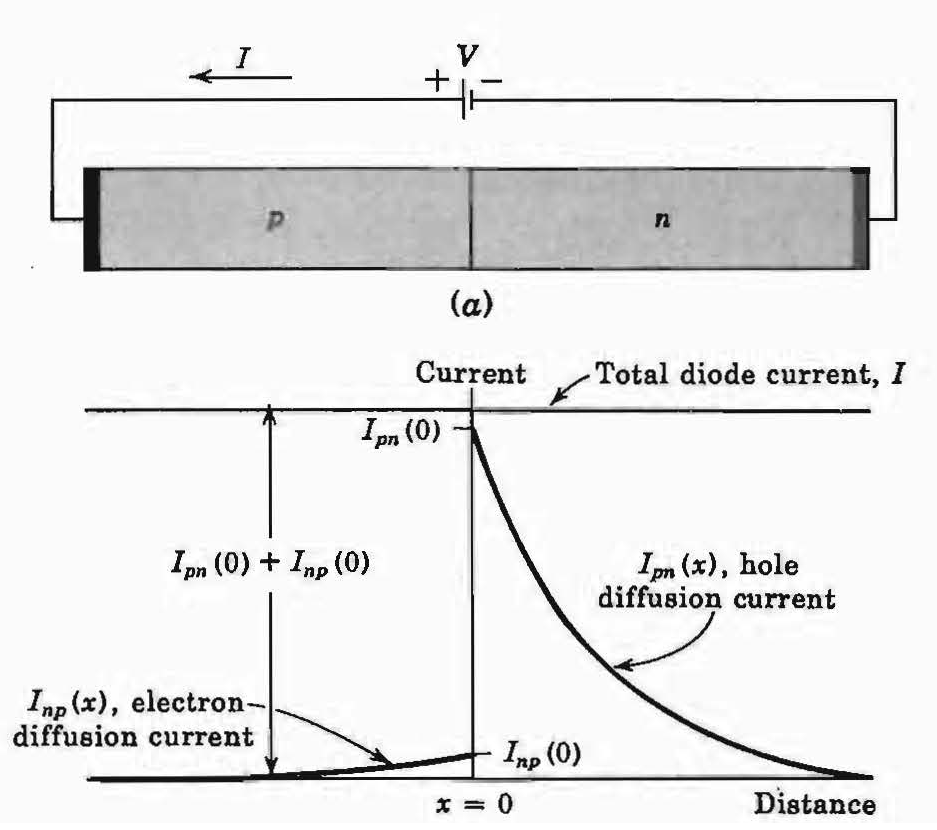
\includegraphics[scale=0.325]{fig/lec03/current_component_in_pn_junction.png}
		\caption{The hole- and electron-current diffusion components vs. distance in a p-n junction diode; adapted from Millman, J., \& Halkias, C. C. Integrated Electronics: Analog and Digital Circuits and Systems.}
		\label{fig:plot_of_pn_junction_current}
	\end{figure}
\end{column}
\end{columns}
\end{frame}

\begin{frame}{Minority Currents in a \textit{p-n} Junction}
	\begin{itemize}
\item Minority carrier current in $n$-type region:
\begin{equation} \label{eq:minority_current_n_region}
	I_{pn}(0) = \frac{AqD_p}{L_p} \left[ p_n(0) - p_{n0} \right]
\end{equation}
where:
\begin{itemize}
	\item $D_p$ = hole diffusion coefficient
	\item $L_p$ = hole diffusion length
	\item $p_n(0)$ = hole concentration at $x = 0$
	\item $p_{n0}$ = equilibrium minority hole concentration
\end{itemize}
\item From law of the junction:
\begin{equation} \label{eq:law_of_junction}
	p_n(0) = p_{n0} e^{\frac{V}{V_T}} \quad
\end{equation}
\end{itemize}

\end{frame}

\begin{frame}{Minority Currents in a \textit{p-n} Junction}
	\begin{itemize}
	\item Substituting Eq. \ref{eq:law_of_junction} into Eq. \ref{eq:minority_current_n_region} gives:
	\begin{equation}
		I_{pn}(0) = \frac{AqD_p p_{n0}}{L_p} \left( e^{\frac{V}{V_T}} - 1 \right)
	\end{equation}

	\item Similarly for electron diffusion:
	\begin{equation}
		I_{np}(0) = \frac{AqD_n n_{p0}}{L_n} \left( e^{\frac{V}{V_T}} - 1 \right)
	\end{equation}

	\item \textbf{Total diode current:}
	\begin{equation}
		I = I_0 \left( e^{\frac{V}{V_T}} - 1 \right)
	\end{equation}
	where:
	\begin{equation*}
		I_0 = \frac{Aq}{L_p} D_p p_{n0} + \frac{Aq}{L_n} D_n n_{p0}
	\end{equation*}
	\item $I_0$ is the reverse saturation current.
	\end{itemize}
\end{frame}	

	
\begin{frame}{Majority Carrier Currents and Total Current Distribution}
	\begin{columns}
		\begin{column}{0.225\textwidth}
	\textbf{Current Continuity and Carrier Profile:}
	\begin{itemize}
		\item Under forward bias, minority carrier current varies with $x$:
		\begin{itemize}
			\item $I_{pn}(x)$ (hole current) decreases exponentially in $n$-region.
			\item $I_{np}(x)$ (electron current) decreases exponentially in $p$-region.
		\end{itemize}
	\end{itemize}
\end{column}
		\begin{column}{0.775\textwidth}
	\begin{figure}	
		\centering
		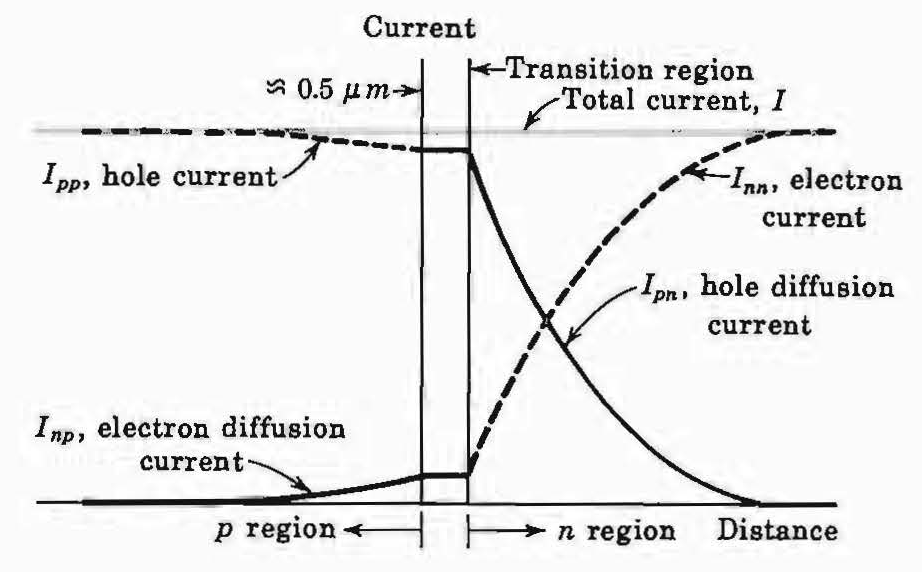
\includegraphics[scale=0.325]{fig/lec03/majority_and_minority_vs_distance.png}
		\caption{The minority (solid) end the majority (dashed) currents vs. distance
		in a p-n diode. lt is assumed that no recombination takes place in the very	narrow depletion region.; adapted from Millman, J., \& Halkias, C. C. Integrated Electronics: Analog and Digital Circuits and Systems.}
		\label{fig:minority_and_majority_current}
	\end{figure}
	\end{column}
	\end{columns}
\end{frame}


\begin{frame}{Majority Carrier Currents and Total Current Distribution}
\begin{itemize}
\item \textbf{To maintain constant total current $I$ across the junction:}
\begin{equation}
	I_{nn}(x) = I - I_{pn}(x), \quad I_{pp}(x) = I - I_{np}(x)
\end{equation}
where:
\begin{itemize}
	\item $I_{nn}(x)$ is majority (electron) current in $n$ region
	\item $I_{pp}(x)$ is majority (hole) current in $p$ region
\end{itemize}

\item \textbf{Total current is bipolar in nature}:
\begin{itemize}
	\item Composed of hole and electron contributions
	\item Varies spatially due to recombination
\end{itemize}
\item Transition region assumed to have negligible recombination width (valid for Si)
\end{itemize}
\end{frame}

	\begin{frame}{Volt-Ampere Characteristic of a \textit{p-n} Diode}
	\textbf{General Current Equation:}
	\begin{equation}
		I = I_0 \left( e^{\frac{V}{\eta V_T}} - 1 \right)
	\end{equation}
	\begin{itemize}
		\item $I_0$ = reverse saturation current
		\item $V$ = applied voltage
		\item $V_T = \frac{kT}{q}$ = thermal voltage ($\approx 26$ mV at 300 K)
		\item $\eta$ = ideality factor ($\approx 1$ for Ge, $\approx 2$ for Si)
	\end{itemize}
	
	\textbf{Interpretation:}
	\begin{itemize}
		\item For $V \gg V_T$: exponential current rise (forward bias)
		\item For $V < 0$: $I \approx -I_0$ (reverse saturation current)
	\end{itemize}

\end{frame}


\begin{frame}{\textbf{Reverse Saturation Current and Breakdown Behavior}}
	\begin{columns}
		\begin{column}{0.25\textwidth}
    	\begin{itemize}
        \item \textbf{Reverse Saturation Current} ($I_0$):
        \begin{itemize}
            \item For reverse bias $V < 0$, diode current saturates to $I = -I_0$.
            \item $I_0$ is weakly dependent on reverse voltage.
            \item Caused by thermally generated minority carriers.
            \item Germanium diodes have $I_0$ \textasciitilde{}1000x larger than silicon.
        \end{itemize}
	\end{itemize}
		\end{column}
		\begin{column}{0.75\textwidth}
	\begin{figure}
		\centering
		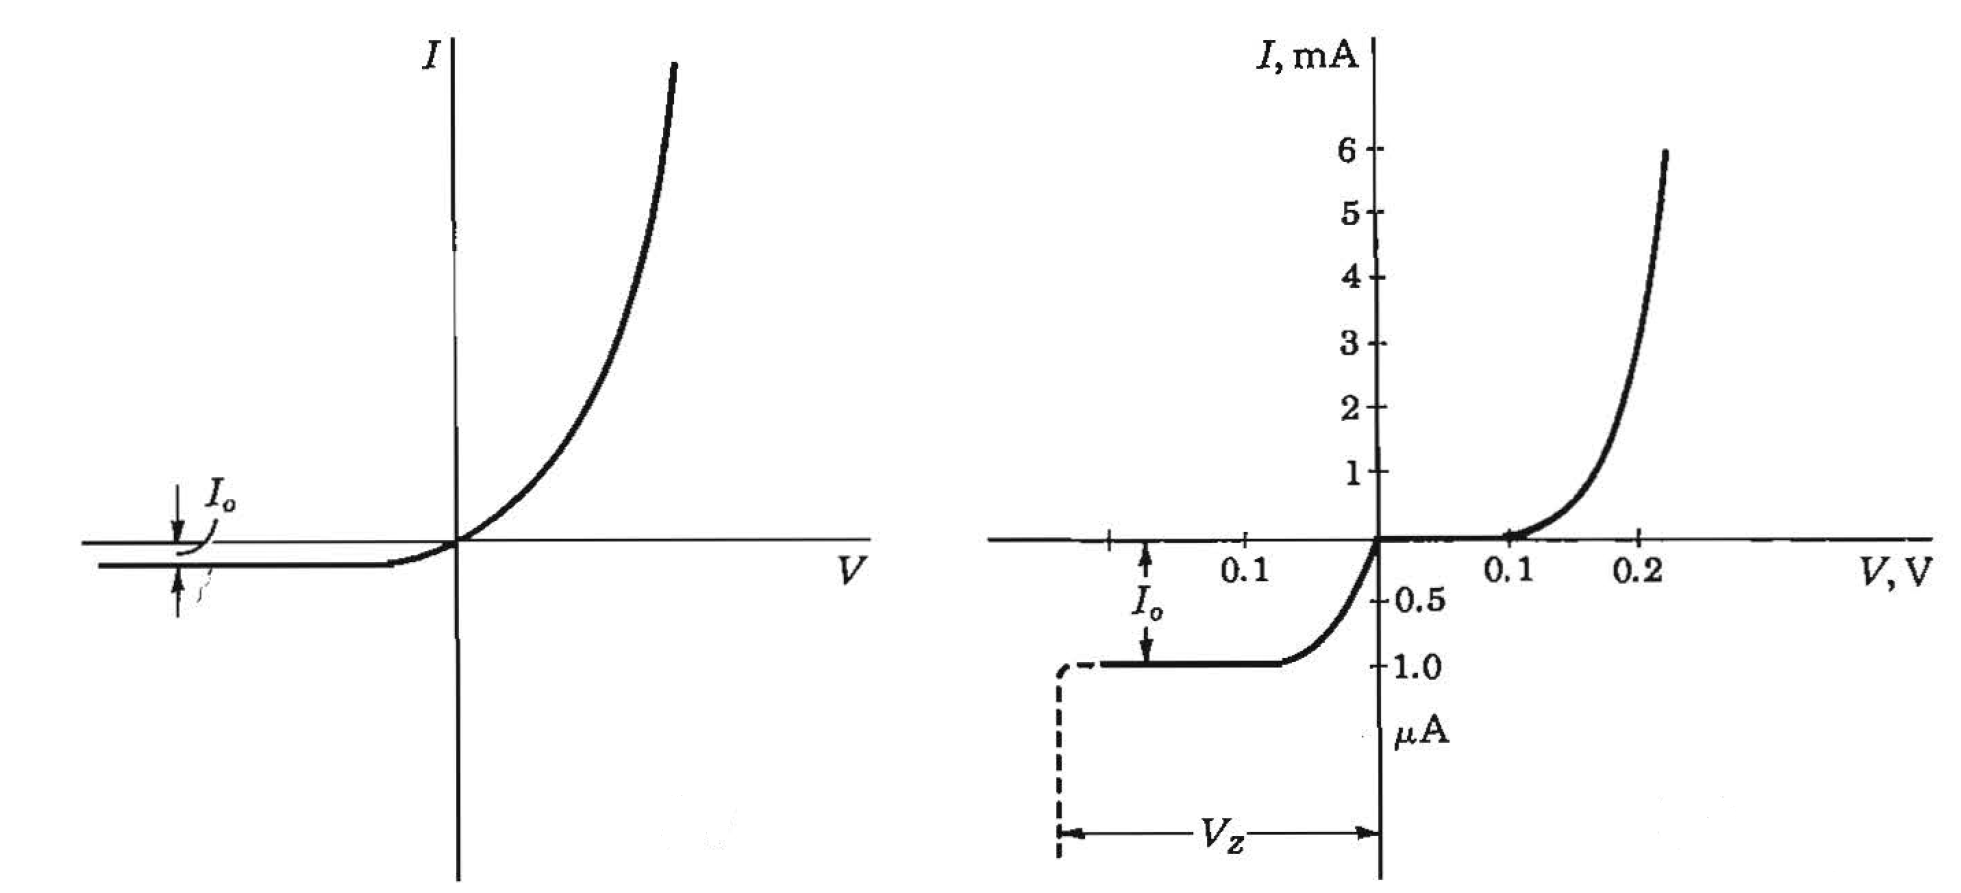
\includegraphics[scale=0.25]{fig/lec03/VI_characteristics.png}
		\caption{The volt-ampere characteristic of an ideal p-n diode and the volt-ampere characteristic for a germanium; adapted from Millman, J., \& Halkias, C. C. Integrated Electronics: Analog and Digital Circuits and Systems.}
		\label{fig:diode_characteristics}
	\end{figure}
	\end{column}
	\end{columns}
\end{frame}

\begin{frame}{\textbf{Reverse Saturation Current and Breakdown Behavior}}
	\begin{columns}
		\begin{column}{0.225\textwidth}
\begin{itemize}
	\item \textbf{Breakdown Region:}
	\begin{itemize}
		\item At a reverse voltage $V_Z$, breakdown occurs $\Rightarrow$ sudden increase in $I$.
		\item Caused by impact ionization or Zener effect.
		\item Fig. 3-6b illustrates abrupt transition at $V_Z$.
	\end{itemize}
\end{itemize}
\end{column}
\begin{column}{0.775\textwidth}
	\begin{figure}
		\centering
		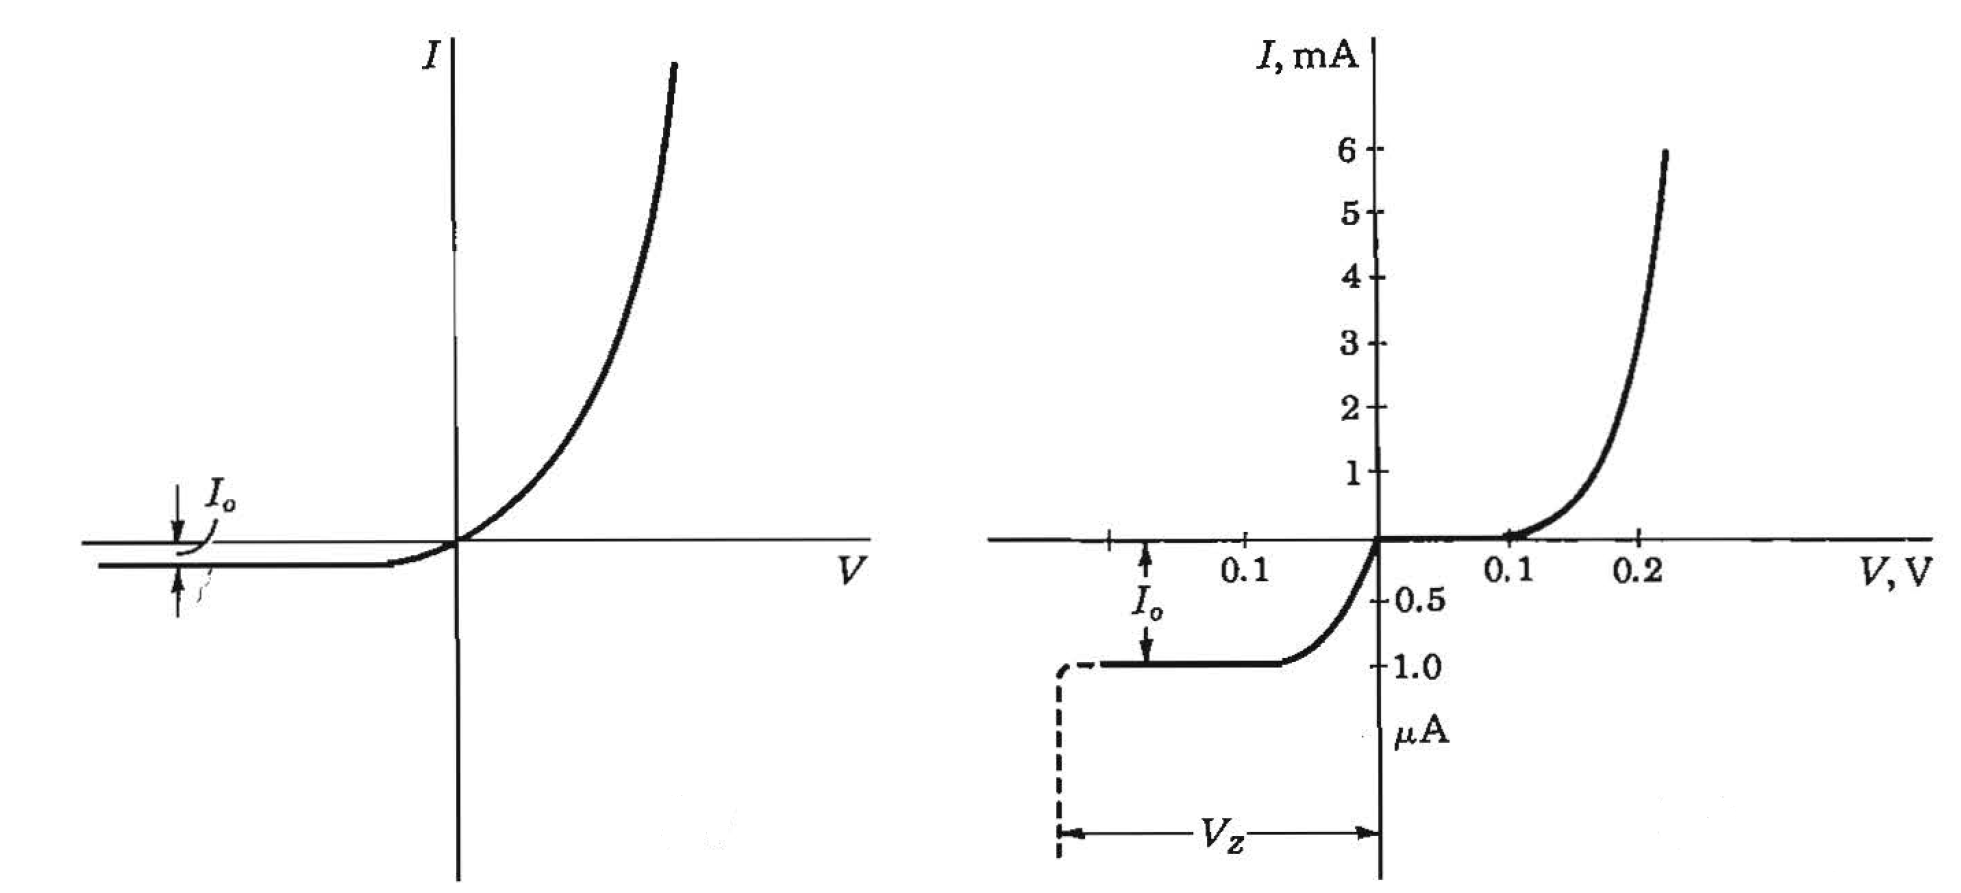
\includegraphics[scale=0.25]{fig/lec03/VI_characteristics.png}
		\caption{The volt-ampere characteristic of an ideal p-n diode and the volt-ampere characteristic for a germanium; adapted from Millman, J., \& Halkias, C. C. Integrated Electronics: Analog and Digital Circuits and Systems.}
		\label{fig:diode_characteristics}
	\end{figure}
	\end{column}
	\end{columns}
\end{frame}



\begin{frame}{\textbf{Cut-in Voltage and Material Comparison}}
	\begin{columns}
		\begin{column}{0.35\textwidth}
    \begin{itemize}
        \item \textbf{Cut-in / Threshold Voltage ($V_\gamma$):}
        \begin{itemize}
            \item Minimum forward bias for noticeable current.
            \item Typically $V_\gamma \approx 0.2$ V (Ge), $\approx 0.6$ V (Si).
            \item Beyond $V_\gamma$, current increases rapidly $\Rightarrow$ exponential growth.
        \end{itemize}
	\end{itemize}
\end{column}
\begin{column}{0.65\textwidth}
	\begin{figure}
		\centering
		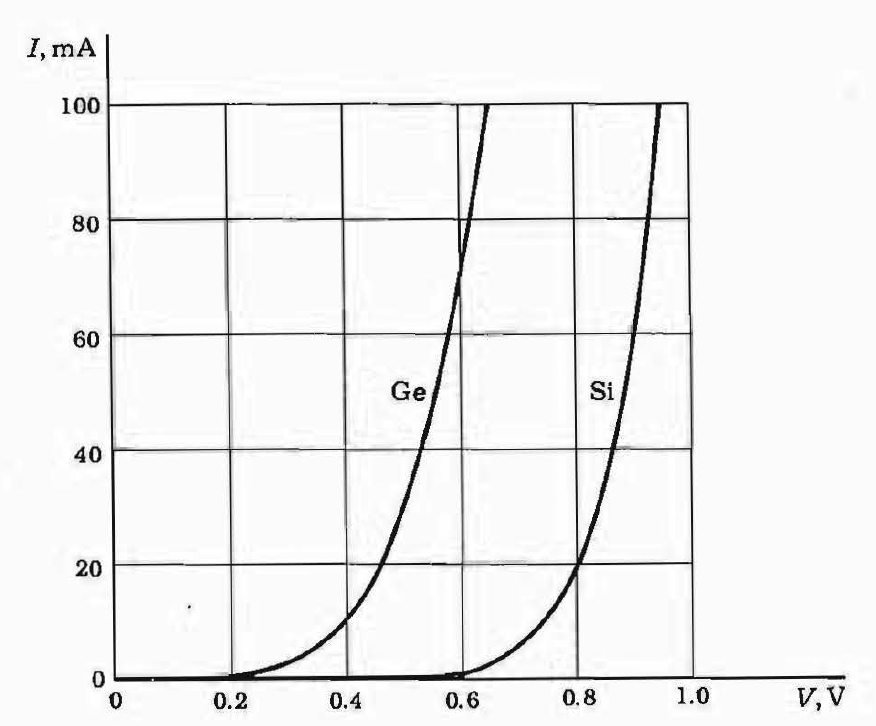
\includegraphics[scale=0.25]{fig/lec03/VI_character_Si_Ge.png}
		\caption{Forward VI characteristics of Si and Ge; adapted from Millman, J., \& Halkias, C. C. Integrated Electronics: Analog and Digital Circuits and Systems.}
		\label{fig:Si_Ge_diode_characteristics}
	\end{figure}
	\end{column}
	\end{columns}
\end{frame}


\begin{frame}{\textbf{Cut-in Voltage and Material Comparison}}
	\begin{columns}
		\begin{column}{0.35\textwidth}
    \begin{itemize}
        \item \textbf{Material Differences:}
        \begin{itemize}
            \item Ge diodes: Lower $V_\gamma$, larger $I_0$, steeper characteristics.
            \item Si diodes: Higher $V_\gamma$, lower $I_0$, more thermal stability.
        \end{itemize}
        \item \textbf{Fig. \ref{fig:Si_Ge_diode_characteristics}:} Comparative $I$-$V$ of 1N270 (Ge) vs 1N3605 (Si).
    \end{itemize}
\end{column}
\begin{column}{0.65\textwidth}
	\begin{figure}
		\centering
		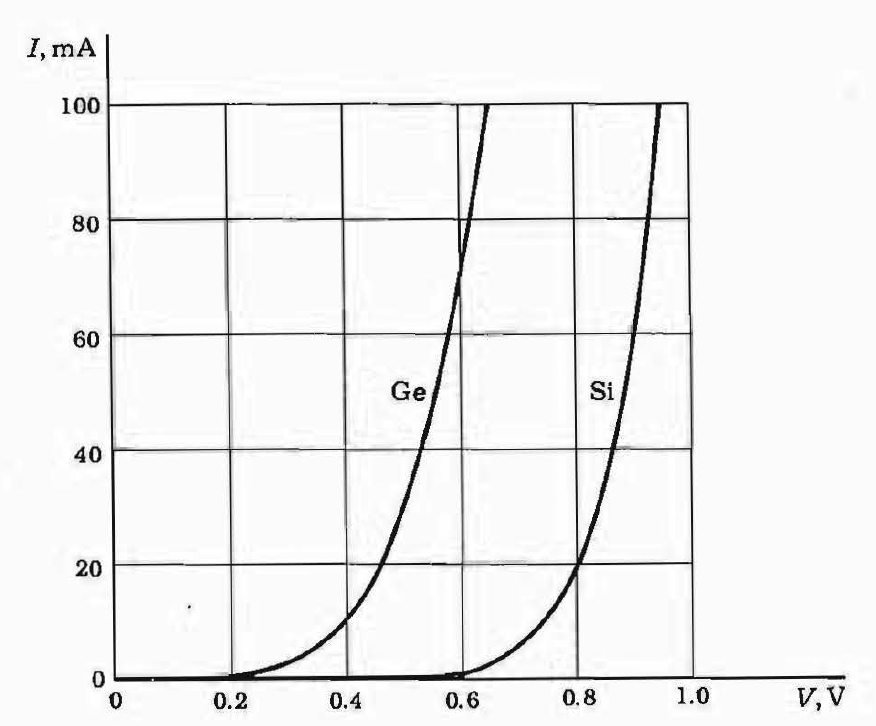
\includegraphics[scale=0.25]{fig/lec03/VI_character_Si_Ge.png}
		\caption{Forward VI characteristics of Si and Ge; adapted from Millman, J., \& Halkias, C. C. Integrated Electronics: Analog and Digital Circuits and Systems.}
		\label{fig:Si_Ge_diode_characteristics}
	\end{figure}
	\end{column}
	\end{columns}
\end{frame}

\begin{frame}{\textbf{Temperature Dependence and $I_0$}}
	\begin{columns}
		\begin{column}{0.5\textwidth}
    \begin{itemize}
        \item $I_0$ increases with temperature:
        \begin{itemize}
            \item $I_0(T) = I_{01} \times 2^{(T - T_1)/10}$
            \item $\Rightarrow$ doubles for every $10^\circ$C rise.
        \end{itemize}
        \item \textbf{Thermal Impact:}
        \begin{itemize}
            \item $V_T = \frac{T}{11600}$ V
            \item At room temp ($300K$), $V_T = 26$ mV
            \item $\left|\frac{dV}{dT}\right| \approx 2.5$ mV/$^\circ$C
        \end{itemize}
        \item Fig. \ref{fig:temp_Si_diode_characteristics} shows $I$-$V$ shifts with temperature: Higher $T \Rightarrow$ lower $V_\gamma$
    \end{itemize}
\end{column}
\begin{column}{0.5\textwidth}
	\begin{figure}
		\centering
		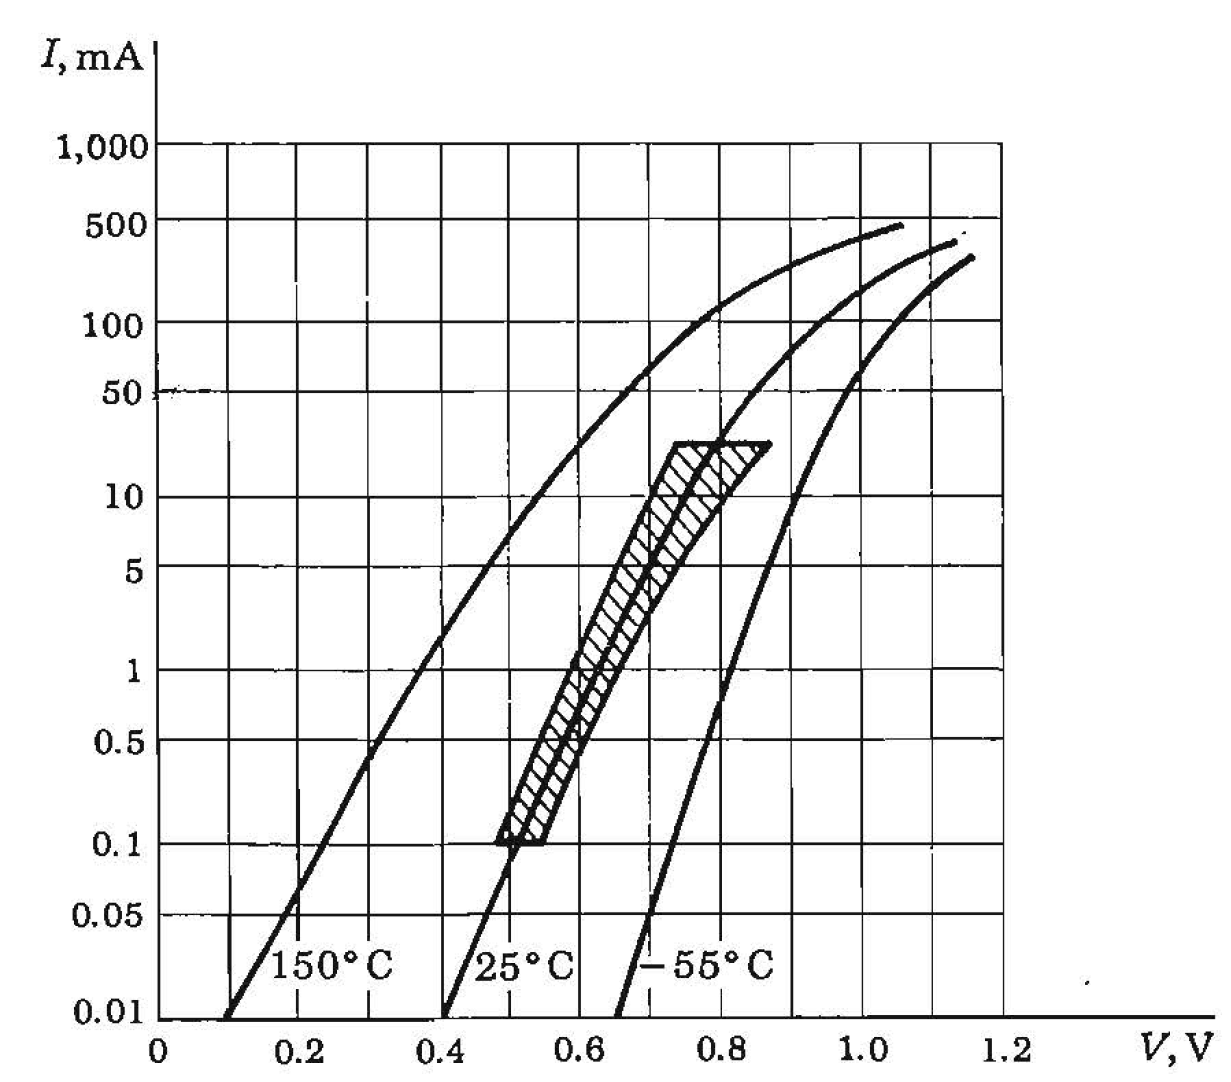
\includegraphics[scale=0.225]{fig/lec03/Temp_dependance.png}
		\caption{VI characteristics at three different	temperatures for a silicon
		diode; adapted from Millman, J., \& Halkias, C. C. Integrated Electronics: Analog and Digital Circuits and Systems.}
		\label{fig:temp_Si_diode_characteristics}
	\end{figure}
	\end{column}
	\end{columns}
\end{frame}

\begin{frame}{\textbf{Diode Resistance and Piecewise Linear Model}}
    \begin{itemize}
        \item \textbf{Static Resistance:} $R = V/I$ \textemdash{} not reliable.
        \item \textbf{Dynamic Resistance:}
        \begin{equation*}
            r = \frac{\eta V_T}{I}
        \end{equation*}
        \item \textbf{Dynamic Conductance:}
        \begin{equation*}
            g = \frac{1}{r} = \frac{I + I_0}{\eta V_T}
        \end{equation*}
        \item \textbf{Piecewise Linear Model:}
        \begin{itemize}
            \item Diode \textasciitilde{} open circuit if $V < V_\gamma$
            \item For $V > V_\gamma$: $r = dV/dI$ constant $\Rightarrow$ $R_f$
            \item Fig. \ref{fig:diode_characteristics}: Diode modeled with $V_\gamma$ and slope $1/R_f$
        \end{itemize}
    \end{itemize}
\end{frame}

\begin{frame}{\textbf{Transition Capacitance ($C_T$)}}
    \begin{itemize}
        \item Under reverse bias, depletion region widens $\Rightarrow$ increase in uncovered charge.
        \item Defined as:
        \begin{equation*}
            C_T = \left| \frac{dQ}{dV} \right|
        \end{equation*}
        \item \textbf{Corresponding Current:}
        \begin{equation*}
            i = C_T \frac{dV}{dt}
        \end{equation*}
        \item $C_T$ is voltage dependent, unlike a linear capacitor.
        \item Important in high-frequency and switching circuits.
    \end{itemize}
\end{frame}


\begin{frame}{\textbf{Diffusion Capacitance: Concept and Static Derivation}}
	\begin{itemize}
		\item \textbf{When forward biased:}
		\begin{itemize}
			\item Excess charge is injected into the neutral region.
			\item Results in large capacitance — called \textbf{diffusion capacitance}, $C_D$.
		\end{itemize}
		
		\item \textbf{Definition:}
		\[
		C_D = \left. \frac{dQ}{dV} \right|_{\text{forward bias}} \quad \text{(rate of change of stored charge w.r.t. voltage)}
		\]
	
		\item \textbf{Using:}
		\begin{align*}
			C_D &= \tau \frac{dI}{dV} = \tau g = \frac{\tau}{r} \tag{3-27} \\
			\Rightarrow C_D &= \frac{\tau I}{\eta V_T} \tag{3-28}
		\end{align*}
		\item Here:
		\begin{itemize}
			\item $\tau$ = carrier lifetime (mean time minority carrier remains mobile)
			\item $I$ = diode current (assumed due to holes)
			\item $\eta$ = ideality factor ($\approx 1$ for Ge, $\approx 2$ for Si)
			\item $V_T = \frac{kT}{q}$ = thermal voltage
		\end{itemize}
	\end{itemize}
	\end{frame}

	\begin{frame}{\textbf{Dynamic Diffusion Capacitance: Arbitrary and Sinusoidal Inputs}}
		\begin{itemize}
			\item \textbf{Implication:} $C_D \propto I$ (linearly dependent on current)
	
			\item \textbf{Time constant:}
			\begin{equation}
			r C_D = \tau \tag{3-29}
			\end{equation}
			where $r = \eta V_T / I$ is the diode dynamic resistance.
			\item \textbf{In general:}
			\begin{equation}
			i = \frac{dQ'}{dt} = C_D' \frac{dV}{dt} \tag{3-30}
			\end{equation}
			\item $C_D' < C_D$ when input varies rapidly.
		
			\item \textbf{Dynamic capacitance:}
			\begin{equation}
			i \neq \frac{dQ}{dt}, \quad i \neq C_D \frac{dV}{dt} \tag{3-31}
			\end{equation}
			since $Q'$ accounts only for instantaneously injected charge, not steady-state.
		\end{itemize}
	\end{frame}	


	\begin{frame}{\textbf{Dynamic Diffusion Capacitance: Arbitrary and Sinusoidal Inputs}}
		\begin{itemize}			
				\item \textbf{For sinusoidal voltage input:}
				\begin{itemize}
					\item Low frequency ($\omega \tau \ll 1$):
					\begin{equation}
					C_D' = \frac{1}{2} \tau g \tag{3-32}
					\end{equation}
					\item High frequency ($\omega \tau \gg 1$):
					\begin{equation}
					C_D' = \left( \frac{\tau}{2\omega} \right)^{1/2} g \tag{3-33}
					\end{equation}
					\item $g = dI/dV = \text{diode conductance}$
				\end{itemize}
			
				\item \textbf{Key Insight:}
				\begin{itemize}
					\item $C_D'$ is frequency-dependent.
					\item Decreases as frequency increases.
					\item Must solve continuity equations to fully describe $C_D'(x,t)$ under general conditions.
				\end{itemize}
		\end{itemize}
	\end{frame}	